\chapter{Quellen des späten Westjiddischen}\label{chap:quellenkapitel}
 % \epigraph{\textit{Historical documents survive by chance, not by design}}{--- \cite[11]{Labov2010}}
  
  \noindent Die Westjiddistik steht, da sie sich um die Erforschung einer ausgestorbenen, historischen Sprache bemüht, in Abhängigkeit zu den uns überlieferten Quellen (vgl.\, \citealt{Weinreich1953}). Die meisten Arbeiten zum späten Westjiddischen konzentrieren sich auf die Dokumentation und Beschreibung des gesprochenen, noch vitalen (West-)Jiddischen nach der Schoah. So z.\,B.\, die Atlasprojekte von \cite{GuggenheimGruenberg1973}, \cite{Beraneck1965}\footnote{\citeauthor{Beraneck1965}s \qu{Westjiddischer Sprachatlas} ist aufgrund \qu{zweifelhafte[r] Ergebnisse und methodische[r] Fehlgriffe} (\citealt[1020]{Katz1983}) als fragwürdige wissenschaftliche Leistung zu beurteilen (vgl.\, \citealt{GuggenheimGruenberg1966b,GuggenheimGruenberg1968}; \citealt[1377—1378]{Althaus1972}; \citealt[1020]{Katz1983}).} und der  von Uriel Weinreich begründete Atlas \qu{Language and Culture Atlas of Ashkenazic Jewry} (\citealt{Herzog1992} \citeyear{Herzog1992,Herzog1995,Herzog2000}; zum \hai{{\WJ}} besonders \citealt{Zuckerman1969}). Diese Arbeiten konnten jedoch nur mehr die vitalen Varietäten des Elsass, der Schweiz und von Teilen Südbadens erfassen. Generell gilt, dass der Raum des westl. \hai{{\SWJ}} besonders überrepräsentiert ist, was die Quellenlage, aber auch was die wissenschaftlichen Arbeiten betrifft \,%rs anstelle von "was… betrifft" in Hinblick auf sowohl…als auch
  (vgl.\, \citealt{Weiss1896,GuggenheimGruenberg1958,GuggenheimGruenberg1966,GuggenheimGruenberg1973,GuggenheimGruenberg1976,GuggenheimGruenberg1981,Zuckerman1969,Brosi1990,Fleischer2004,Fleischer2004b,Fleischer2005,Schaefer2008,Schaefer2014}{; }\citealt{Weisskirchen2011}). Zum \hai{{\ZWJ}} gibt es hingegen nur einige wenige lexikalische Arbeiten, die sich meist auch nur auf jiddische Lehnwörter in den deutschen Dialekten stützen (\citealt{Frank1962,Weinberg1973,Althaus1963,Post1992,Klepsch2004}). Aber nur die Arbeiten von \cite{Frank1962} (\hai{{\ZWJ}}) und \cite{Weinberg1973} (\hai{{\NWJ}}) beruhen auf Interviews mit Muttersprachlern und/oder mit der nachfolgenden Generation der letzten Sprecher des Westjiddischen. Unser Wissen zum \hai{{\NWJ}} basiert überwiegend auf Untersuchungen  literarischer Quellen (vgl.\,\citealt{Landau1901,Reershemius2007,Reershemius2014,Schaefer2013}). Zum niederländischen \hai{{\NWJ}} liegen Untersuchungen zur Lexik und Phonologie vor (\citealt{VanGinneken,VoorzangerPolak1915,Beem1954,Beem1970,Beem1974,Beem1975,Aptroot1991,Aptroot2002}). Forschungsbedarf besteht im östl. \hai{{\SWJ}} sowie in den Übergangszonen. Immerhin zum ungarischen Jiddischen liegen uns \,%rs Zum ungarischen Jiddischen liegen uns immerhin
  die Arbeiten \citeauthor{Hutterer1965}s (\citeyear{Hutterer1965,Hutterer1994}) und \citeauthor{Garvin1965}s (\citeyear{Garvin1965}) vor. Auch das \hai{{\NÜJ}} ist in \cite{Herzog1965} gut erfasst. Zum Jiddisch im \ili{tschechisch}-slowakischen Sprachgebiet sind die Arbeiten \citeauthor{Trost1965}s (\citeyear{Trost1965}) und Beraneks (\citeyear{Beranek1936,Beranek1949}) unsere einzigen Quellen. Eine Zusammenstellung der Quellen zum Burgenländer Jiddisch findet sich neben einer knappen Darstellung der sprachlichen Eigenschaften in \textcite{Schaefer2017}.

Doch birgt die Quellenlage zum Westjiddischen noch immer Analysepotential für weitere Arbeiten. So nennt \cite{Weinreich1953} eine Vielzahl literarischer Quellen jüdischer wie christlicher Autoren, die uns Auskunft über den Zustand des Westjiddischen im 18. und 19. Jahrhundert liefern können. Bereits Landaus Analyse der Memoiren der Glikl bas Judah Leib kann als erster Versuch gelten, Reflexe des umgangssprachlichen Jiddischen in einem literarischen Text nachzuweisen (\citealt{Landau1901}). Mit den Arbeiten von \cite{AptrootGruschka2004}, Reershemius (\citeyear{Reershemius2007,Reershemius2014}), \cite{Weisskirchen2011}, \cite{FleischerSchaefer2012} und \citeauthor{Schaefer2008} (\citeyear{Schaefer2008,Schaefer2010,Schaefer2013,Schaefer2014}) mehren sich in jüngster Zeit Analysen des Westjiddischen, die auf literarischen Quellen des 19. Jahrhunderts fußen und damit erstmals den Sprachstand jener Zeit erfassen.

Diesem Trend folgt auch das von der Deutschen Forschungsgemeinschaft geförderte Projekt \qu{\ili{Westjiddisch} im (langen) 19. Jahrhundert: Quellenlage, soziolinguistische Situation und grammatische Phänomene} an der Philipps-Universität Marburg. In diesem Projekt wurde zwischen 2011 und 2016 in erster Linie daran gearbeitet, einen Gesamtüberblick der Quellenlage zu gewinnen. Daran anschließend werden einzelne, besonders ergiebige Quellen betreffs ausgewählter sprachlicher Phänomene analysiert und beschrieben (\citealt{Weisskirchen2011,Schaefer2013,Schaefer2014}{; }\citealt{FleischerSchaefer2012}). Die nachfolgenden Abschnitte beruhen auf dem in diesem Projekt erarbeiteten Quellsample und auf ersten daraus gewonnenen Ergebnissen.\footnote{Der dieser Arbeit zu Grunde liegende Stand des Projektsamples ist der vom 03. Oktober 2013. Eine regelmäßig aktualisierte Version des Projektsamples ist unter \url{http://www.online.uni-marburg.de/westjiddisch/} einsehbar und durchsuchbar. Die folgenden Histogramme erfassen 276 Quellen, da zu dreien kein Erscheinungsdatum eruiert werden konnte. Die Erschließung von Quellen erfolgt im Projekt über Recherchen in Judaica-Beständen von Bibliotheken und gezielte Suchabfragen in digitalen Beständen durchsuchbarer Textzeugen des (langen) 19. Jahrhunderts. Die Erfüllung/Nichterfüllung sprachlicher Charakteristika des Westjiddischen (z.\,B.\, Kennwörter wie \textit{Ette} \sem{Vater}, \textit{Memme} \sem{Mutter} oder vokalische Strukturen wie {\mhd} \textit{ei}/\textit{ou} als <aa>) entschieden dabei über die Aufnahme von Texten in das Projektsample.}

 
 
 
 
 \section{Der jüdische Multilingualismus}\label{multilingualismus}%LS dieses Kapitel habe ich etwas umgeschrieben
%\noindent
Die jüdischen Kulturen der Diaspora bewegen sich in einem Spannungsfeld  zwischen zwischen As­si­mi­la­ti­on an die jeweiligen koterritorialen Kulturen und der Bewahrung der eigenen kulturellen Identität (Dis­si­mi­la­ti­on). Diese Problematik spiegelt sich auch in den jüdischen Sprachen wieder. Das Judentum der Diaspora hat allein aufgrund der Dichotomie zwischen Alltags- und Sakralsprache immer eine bi- bzw. multilinguale Ausrichtung (vgl.\, \citealt{Weinreich1962,Mieses1915,Fischer1936}). Die Alltagssprache, insbesondere die der innerjüdischen Kommunikation, ist das Jiddische. Darüber hinaus kann man beim aschkenasischen Judentum einen Bidialektalismus nicht-jüdischer Dialekte (d.\,h. gesprochensprachlicher Varietäten) feststellen (\citealt{Weinreich1962,Schaefer2008,Schaefer2014}{; } s.\,a. \qu{Die Hochzeit zu Grobsdorf} 1822:\,2–7 in \citealt{Lowenstein1975}). Dies gilt sowohl für den ost- als auch für den westjiddischen Sprachraum. Im westjiddischen Gebiet ist zudem in der Schriftlichkeit eine Ausrichtung an deutschen Literatursprachen zu verzeichnen, die auf schriftdeutsche Varietäten der jüdischen Bevölkerung hinweisen. Der Unterschied zwischen dem Deutsch von Juden und dem von Christen darf als äußerst gering eingeschätzt werden. In der Regel handelt es sich lediglich um eine orthographische Differenz zwischen jüdischem und christlichem Schriftdeutsch (Stichwort: \sem{Deutsch in hebräischen Lettern} s. nachfolgendes Kapitel \ref{Überlieferungsformen}). In Anlehnung an Haïm Vidal Séphiha  (\citeyear[193]{Sephiha1985}) und Paul Wexler (\citeyear[7]{Wexler1987}) bezeichne ich diese Varietäten als Judeo-X-Sprachen.
Ich unterscheide jedoch zwischen zwei Typen von Judeo-X-Sprachen. Typ 1 der Judeo-X-Sprachen zeichnet sich dadurch aus, dass hier keine von der X-Sprache eigenständigen grammatischen Strukturen vorliegen und sich die Judeo-X-Sprachen lediglich auf Basis von kulturell bedingten Lexemen, welche zumeist aus der \ili{hebräisch}-aramäischen Komponente stammen, von der koterritorialen X-Sprache unterscheiden. Im Typ 2 hingegen bestehen eigenständige grammatische Strukturen der Judeo-Sprache gegenüber der X-Sprache, wie dies im Jiddischen der Fall ist. Ein weiterer Typ jüdischer Varietäten sind die auf hebräischer Lexik (und z.\,T. \isi{Morphologie}), aber auf germanischer \isi{Syntax} basierenden Sondersprachen, die auch koterritoriale Sondersprachen (insbes. rotwelsche Sprachen) beeinflusst haben (vgl.\, \citealt{GuggenheimGruenberg1981,Matras1996}).

Das nachfolgende Schema zeigt den jüdischen Multilingualismus, der sich auf einer Skala zwischen koterritorialer Kultursprache (\isi{Assimilation}) und jüdischer Sakralsprache (Dissimilation) verteilt.\footnote{Für die tatsächliche Sprachrealität ist allerdings anzunehmen, dass nur in seltenen Einzelfällen ein Individuum alle fünf Varietäten beherrscht hat.} %Besonders die Varietäten \hai{A.} und \hai{D.} sind in der jüdischen Diaspora eher selten zu finden. 


 
 \begin{description}\label{schämamultilingualismus}
  
  \item [\isi{Assimilation}/X-Sprachen]
  
  \item [A] Koterritoriale Varietäten

  \item [B] Judeo-X-Sprachen; vgl.\, \citet[193]{Sephiha1985}
  
\begin{itemize}
\item [\hai{Typ 1}] ohne von X-Sprache losgelöster Grammatik, lexikalisch markiert,\\ z.\,B.\, \textit{Judeo-Englisch}, \textit{Judeo-German}\footnote{Für den deutschsprachigen Raum ließe sich vom Judeo-German bzw. vom problematischen, weil anderweitig besetzten Terminus \textit{Jüdisch-Deutsch} sprechen (vgl.\, \citealt{FleischerimErsch}).} %format! prüfen: passt die FN hier?
\item [\hai{Typ 2}] mit von X-Sprache losgelöster Grammatik,\\ z.\,B.\, \textit{Karaimisch} (Trakei), \textit{\alert{Jiddisch}}

\end{itemize}  
 
\item [C] Hebraeo-X–Sprachen\\
 Sonder- oder Geheimsprachen,
 z.B. Händlersprachen

\item [D] Hebräisch-aramäische Varietäten\\
z.\,B.\, \textit{Ivrit}

\item[Dissimilation/Sakralsprache]

  \end{description}%AA


Dieser kurze Blick auf die jüdische Sprachsituation der Diaspora macht zweierlei deutlich: Zum einen ist Jiddisch eine jüdische Varietät unter vielen und zum anderen fungiert Jiddisch (insbes. \ili{Westjiddisch}) innerhalb dieses Varietätennetzes vorwiegend als gesprochene Sprache zur Alltagskommunikation. Eine Verschriftlichung dieser Varietät stünde somit nicht nur außerhalb ihrer natürlichen, also mündlichen, Funktion, sondern spräche auch dafür, dass das ursprüngliche Gleichgewicht zwischen Schreib- und Sprachvarietäten gestört ist. Wie das nachfolgende Kapitel zeigt, tritt die Verschriftlichung des gesprochenen Jiddischen in einer Phase der aschkenasischen Geschichte auf, in der wir einen Einbruch alter Schreibtraditionen feststellen können.
 
 
 
 
 \section{Überlieferungsformen des Westjiddischen}\label{Überlieferungsformen}
 \largerpage[-1]
 %\noindent
Die westjiddische Sprachsituation im 19. Jahrhundert generiert nach \citeauthor{Lowenstein1979} drei schriftsprachliche Systeme  (\citealt[180]{Lowenstein1979}) :   

 \begin{description}
  \item [I. Old literary Yiddish] in Hebrew script
  \item [II. High German in Hebrew script]  %(\textit{Jüdisch-deutsch})
  \item [III. Yiddish dialect] (i.) in Hebrew script, (ii.) in Latin script  
  \end{description}

\noindent Unter \qu{Old literary Yiddish} \,%rs old groß
versteht \cite[179]{Lowenstein1979} \qu{a literary language which was a compromise between the spoken dialects of Eastern and Western Europe}. Dieses System einer Ausgleichssprache zwischen Ost- und \ili{Westjiddisch} findet sich bereits ab mitteljiddischer Zeit (\citealt[17]{Kerler1999}). Mit dem Erstarken des Ostjiddischen und der Aufgabe des Westjiddischen im 19. und frühen 20. Jahrhundert verliert dieser Typ an Nutzen. Für den westjiddischen Sprachraum liegen die Alternativen in der Verwendung des Deutschen oder – in seltenen Fällen – des regionalen jiddischen Dialekts.

Deutschsprachige Drucke in hebräischen Lettern (\textit{Ivre-taytsh}) kommen nach \citeauthor{Lowenstein1979} (\citeyear[179--180]{Lowenstein1979}; s.\,a. \citealt[113]{Beider2013}) ab dem späten 18. Jahrhundert auf. In Handschriften findet sich Deutsch in hebräischen Lettern jedoch deutlich früher. Wie zum Beispiel in Handschriften aus dem 17. und 18. Jahrhundert im Archiv des \textit{Genisaprojekts Veitshöchheim} oder auch im Bestand des Hessischen Staatsarchivs Marburg (u.\,a.\, unter der Signatur 340 v. Geyso). \citeauthor{Lowenstein1979} berücksichtigt nicht, dass auch eine Vielzahl jüdischer Publikationen auf Deutsch in lateinischen Lettern bzw. Fraktur existieren. Die Verwendung des Schriftsystems (hebräische vs. lateinische Lettern) variiert tatsächlich nicht nur bezüglich der Verschriftlichung des Jiddischen, sondern auch betreffs des Deutschen. Dies zeigt, dass \citeauthor{Lowenstein1979} ein sehr hohes Gewicht auf den Gebrauch des hebräischen Schriftsystems legt. Die Quellsituation zum Westjiddischen ist jedoch weitaus komplexer und nicht bloß an Schriftsystemen festzumachen. Die alt- und mitteljiddische Literatursprache kann bis zu einem gewissen Grad auch als von deutschen Schreibtraditionen und besonders überregionalen Schreibstilen des Deutschen beeinflusst betrachtet werden.\footnote{Ein eindrucksvolles Beispiel hierfür ist der jüdische Artusroman \qu{Widuwilt} (14./15.–17.Jh.), der nicht nur eine literarische Modeerscheinung der Frühen Neuzeit in die aschkenasische Welt transponiert, sondern insbesondere sprachlich nah am Frühneuhochdeutschen orientiert ist  (vgl.\, \citealt{Jaeger2000,Wolf1974}).}  

Im Gegensatz zum \quein{Deutsch in hebräischen Lettern} des 19. Jahrhunderts ist die Nähe zwischen alt-/mitteljid\-discher und deutscher Literatursprache nicht auf den ersten Blick ersichtlich, doch besonders der Vergleich mit gesprochenen Varietäten des Ost- und Westjiddischen, die sich stark von der schriftlich fixierten alt-/mitteljiddischen Sprache unterscheiden, zeigt, dass bereits vor dem 19. Jahrhundert eine jüdische Schreibtradition bestand, die sich am Deutschen orientierte. Nur war zu diesem Zeitpunkt auch das Schriftdeutsche wesentlich uneinheitlicher als im 19. Jahrhundert. Damit liegt eine Diglossie zwischen jüdischer Schreibvarietät und gesprochener Sprache vor. Eine terminologische Einteilung in Judeo-German (\textit{Jüdisch-Deutsch}; von Juden gesprochenes Deutsch) und \ili{Westjiddisch}, wie sie Fleischer (\citeyear{FleischerimErsch}) für die synchrone Situation des (langen) 19. Jahrhunderts vornimmt, ist auch ein sinnvoller Ansatz für die Diachronie. Man könnte damit von zwei germanischen Varietäten der Juden auf deutschsprachigem Raum ausgehen.\footnote{Im Schema auf S.\, \pageref{schämamultilingualismus} wären dies die Varietäten \hai{B} und \hai{C}.}

Dialektales \ili{Westjiddisch} ist erstmals ab 1780 schriftlich fixiert (\citealt[180]{Lowenstein1979}). Vorwiegend sind uns Dramen überliefert, welche aus der Feder von Maskilim stammen. So kommt es, dass unsere ersten Quellen vom gesprochenen \ili{Westjiddisch} von Autoren stammen, die mit diesen Texten die sprachliche \isi{Assimilation} propagieren und die jiddische Sprache in ihren Texten als Mittel zur Pejoration einsetzten. In vielen Fällen sind diese ersten Quellen auch die letzten Quellen für einen speziellen westjiddischen Dialekt. So zum Beispiel im Fall des im hessischen Raum gesprochenen jiddischen Dialektes, von dem uns nur das Drama \quji{\RL{דיע ה{א\makebox(-1.25,-1.25)[r]{\libertineGlyph{uni05B8}}}כצייט צו גר{א\makebox(-1.25,-1.25)[r]{\libertineGlyph{uni05B8}}}בסד{א\makebox(-1.25,-1.25)[r]{\libertineGlyph{uni05B8}}}רף}} [\qu{Die Hochzeit zu Grobsdorf}] (1822) von Arje Löb Rosenthal als autochthone Quelle eines Muttersprachlers überliefert ist (vgl.\, \citealt{Lowenstein1975}). Alle anderen Quellen  aus dieser Region, wie z.\,B.\, die Friedberger Theaterstücke \qu{Der Judenball im Wäldchen} (zwischen 1858–1865) von G. Emmerich und \qu{Die Gebrüder Haas im Jahre 1848 oder das Loos Nr. 7777}  (1853) von Adolf Müller, sind von christlichen Autoren verfasst und damit von Autoren ohne muttersprachliche Kompetenz des Westjiddischen. 

Dies heißt allerdings nicht zwangsläufig, dass eine Rekonstruktion des gesprochenen Westjiddischen vor 1780 unmöglich ist. Die Quellen des dialektalen Westjiddischen im 19. Jahrhundert können uns wesentliche Vergleichswerte liefern, auf die wir ältere Texte oder Texte anderer Schreibvarietäten prüfen können. Gesprochensprachliche Reflexe sind prinzipiell in allen Schreibvarietäten \citeauthor{Lowenstein1979}s auffindbar. Dabei ist die Einordnung eines Textes als konzeptionell mündlich oder konzeptionell schriftlich (nach \citealt{KochOesterreicher1985}), d.\,h. näher an der gesprochenen bzw. geschriebenen Sprache orientiert, immer graduell. Dies betrifft nicht nur die Quellen des 19. Jahrhunderts, sondern im besonderen Maße auch alt- und mitteljiddische Texte:\footnote{Ein Beispiel für gesprochensprachliche Reflexe findet sich in der Handschrift einer \textit{magischen Zauberformel} von ca.\, 1700 (Transliteration und Scan der Hs. sind im Anhang (S.\, \pageref{part_schirm}) aufgeführt.}

\begin{quote}
Depending on the intention of the author, a text written by an Ashkenazi Jew to be understood by other Jews living in German speaking lands could be modelled on literary German, on spoken language, or on the language of scholars who interspersed their spoken or written Yiddish with many Hebrew and Aramaic words and phrases. (\citealt[117]{Aptroot2010})
\end{quote} 

Reflexe des Westjiddischen lassen sich darüber hinaus auch in nicht-jüdischen Sprachen finden, etwa in deutschen Dialekten (\citealt{Althaus1963,Post1992,Klepsch2004,Stern2000}), modernen Schreibvarietäten (\citealt{Althaus2010}) oder Sondersprachen wie etwa dem Manischen (\citealt{Lerch1976}) oder Lachoudischen (\citealt{Klepsch2004}). Der Einfluss des Jiddischen ist hier jedoch weitestgehend auf die lexikalische Ebene beschränkt und nur in strittigen Einzelfällen zeigt auch die \isi{Morphologie} Reflexe von Interferenzen. Doch nicht nur Varietäten des Deutschen, sondern auch Varietäten jeder beliebigen Sprache, die in einem näheren Kontakt zum Jiddischen stehen, können durch Entlehnungen Formen des Jiddischen reflektieren. Populärstes Beispiel ist das \qu{Jewish English},\footnote{Z.\,T. auch als \textit{Yinglish} bezeichnet.} welches einzelne Jiddismen ins amerikanische Englisch aufnimmt. Vorzugsweise findet sich dies bei Juden mit einem aschkenasischen Hintergrund, es streut aber vermehrt in andere Sprechergruppen aus (u.\,a.\, \citealt{Benor2000,Benor2009,Gold1985,Fishman1985}).  

Wie bereits \cite{Weinreich1953} aufzeigt, können auch literarische Quellen jüdischer wie nicht-jüdischer Autoren Reflexe des gesprochenen Jiddischen aufweisen. Diese Quellen betreffen in erster Linie poetische Texte und die in ihnen umgesetzte sprachliche Markierung jüdischer Figuren. Dieses \hai{{\LiJi}} (\citealt{Richter1995}) erweist sich als eine viel ergiebigere Quelle als weithin angenommen. Es findet sich in unterschiedlichen literarischen Funktionen, was eine weitere Untergliederung dieses Quelltyps erforderlich macht (s. Kapitel \ref{Kapitel Funktionstypen}). Quelltypen mit Reflexen des gesprochenen \ili{Westjiddisch} sind demzufolge: 

\begin{description}
\item [I. Dialektales Jiddisch]  medial mündliche Quellen; ausschließlich aus dem späten westl. \hai{{\SWJ}} in Tonaufnahmen konserviert (\citealt{GuggenheimGruenberg1966,Fleischer2005}).
\item [II. Schreibvarietäten des Jiddischen] jüdische Autorschaft; in hebr. Schrift (z.\,B. die Hs. des Marburger Staatsarchivs; Appendix, S.\, \pageref{part_schirm}).
\item [III. Schreibvarietäten des Deutschen] jüdische Autorschaft; in hebr. u. lat. Schrift.
\item [IV. \ili{Literaturjiddisch}] jüdische u. nicht-jüdische Autorschaft; in hebr. u. lat. Schrift. Jiddisch steht immer in einer literarischen Funktion im Kontrast zu einem Superstrat (hier Deutsch).
\item [V. Entlehnungen aus dem Jiddischen in andere Sprachen] z.\,B.\, in dt. u. {\engl} Varietäten; jüdische und nicht-jüdische Sprecher; in lat. Schrift.
\end{description}

Mit dieser Einteilung verschiebt sich die Definition von dialektalem Jiddisch. Während dieses bei \cite{Lowenstein1979} noch Theaterstücke der Maskilim abdeckt, zähle ich diese zum Literaturjiddischen, da Jiddisch hier eine literarische Funktion trägt. 
  
  
  
    \section{Funktionstypen des Literaturjiddischen} \label{Kapitel Funktionstypen}
	  %  %\noindent
	Auf der Grundlage der im Projekt \qu{\ili{Westjiddisch} im (langen) 19. Jahrhundert} erschlossenen Quellen lassen sich vier Funktionstypen herausfiltern, in denen der jiddischen Sprache unterschiedliche literarische Funktionen zukommen. Jeder Typ ist in zwei Subkategorien zu unterteilen, die die Dichotomie \hai{jüdische vs. christliche Autorschaft} ausdrückt. Diese Zweiteilung entspricht  der Dichotomie \hai{interne vs. externe Sprachwahrnehmung} und reflektiert damit auch die mögliche Sprachkompetenz eines Autors. Die Typisierung westjiddischer Quellen gestaltet sich damit wie folgt. Die verschiedenen Typen sind gleichzeitig als voneinander separiert und voneinander beeinflusst zu betrachten, da sie bis zu einem gewissen Grad auch die Stadien des Jiddisch-Diskurses im deutschsprachigen Raum des 19. Jahrhunderts widerspiegeln (vgl.\, \citealt[55–59]{SchaeferDiss}):\\
	
	
	
	 \begin{description}
	  \item [Funktionstyp A] \hai{autochthon}
	  \item (1) \hai{abbildend}: Autoren sind Muttersprachler; überwiegend Lokalpossen, aber auch metasprachliche Texte (Wörterbücher, Grammatiken), vorwiegend aus dem westl. \hai{{\SWJ}} überliefert; z.\,B.\, \qu{Garkisch} von Josy Meyer (1930) (s.\,a. \citealt{Schaefer2014}). Nur von diesem Texttyp lässt sich mit Gewissheit sagen, dass er ausschließlich an ein jiddischsprachiges Publikum adressiert ist.
	  \item (2) \hai{beschreibend}: Grammatiken, Lehrbücher oder Ausdruckssammlungen christlicher Autoren, z.\,B.\, \qu{Unterricht in der Judensprache, und Schrift} (\citealt{Friedrich1784}). 
	  \item [Funktionstyp B] \hai{pejorativ}
	  \item (1) \hai{jüdische Ablehnung}: jüdische Autoren (mit überwiegend muttersprachlicher Kompetenz) propagieren über die sprachliche \isi{Assimilation} die jüdische Emanzipation, z.\,B.\, Theaterstücke der Maskilim wie Wolfssohns \qu{Leichtsinn und Frömmelei} (1796).
	  \item (2) \hai{christliche Ablehnung}: antisemitische Schriften, z.\,B.\, Sessas polarisierendes Theaterstück \qu{Unser Verkehr} (1816).
	  \item [Funktionstyp C] \hai{humoristisch}
	  \item (1) \hai{jüdische Karikaturen}: Besonders in Großstädten im bürgerlichen Judentum verbreitet, z.\,B.\, die in min. 23 Heften erschienenen \qu{Gedichte und Scherze in jüdischer Mundart} aus Berlin (s.\,a. \citealt{Gruschka2003}). %oder den Amsterdamer \textit{yontev-bletlekh} (\citealt{Aptroot2008}). 
	  \item (2) \hai{christliche Karikaturen}: Breite gesellschaftliche Streuung, z.\,T. latent antisemitisch wie die von Christian Heinrich Gilardone in zwei Bänden erschienenen Sammlungen \qu{Parodiee, Gedichtches unn prousaische Uffsätz} (1. Bd. 1832, 2. Bd. 1835).
	  
	\item [Funktionstyp D] \hai{konservierend–nostalgisch} 
	  \item (1) \hai{historisierende, idealisierende Skizzen jüdischer Autoren}: Die Autoren sind keine aktiven Sprecher/Muttersprachler des Jiddischen (mehr) bzw. schreiben für ein nicht muttersprachliches Publikum, z.\,B.\, Wassermanns \qu{Die Juden von Zirndorf} (1897), aber auch metasprachliche Arbeiten wie Tendlaus \qu{Sprichwörter und Redensarten deutsch-jüdischer Vorzeit} (1860). Diese Quellen können jedoch auch autochthone sprachliche Strukturen reflektieren, wie dies etwa die \qu{Lebenserinnerungen} des A. H. Heymann (1909) zeigen (\citealt{Schaefer2013}).
	  \item (2)  \hai{historisierende, idealisierende Skizzen jüdischen Lebens christlicher Autoren}: Z.\,B. Wilhelm Raabe \qu{Frau Salome} (1879),  Adolf Müller \qu{Die Gebrüder Haas im Jahre 1848 oder das Loos Nr. 7777} (1853).
	 \end{description}


	In zwei Fällen ist die Funktionszuweisung eines Textes jedoch problematisch. Die konkrete Differenzierung zwischen den Funktionen der Typen \hai{B2} und \hai{C2} besteht darin, dass zwar in beiden Fällen antisemitisches Gedankengut transportiert werden kann, jedoch nur in \hai{B2}-Quellen die Textfunktion primär antisemitisch ist, wohingegen antisemitische Sequenzen in \hai{C2} nicht im Bezug zur sprachlichen Markierung stehen,  sondern lediglich zur humoristischen Unterhaltung dienen. Wenn es auch aus  heutiger Sicht schwer nachvollziehbar ist, dient in Texten des \hai{C2}-Typus Antisemitisches der Belustigung des Lesers und nicht der moralischen Degradierung der jüdischen Glaubensgemeinschaft, wie im Fall von \hai{B2}-Texten. Eine klare Trennung zwischen diesen Typen ist aber in vielen Fällen nicht einfach.  Daher wurde für die folgende Auswertung ein gemeinsamer Mischtyp \hai{B2}/\hai{C2} angesetzt. Es ist im Grunde sogar möglich, allen Texten (außer denen vom Typ \hai{A1}) eine mehr oder weniger stark ausgeprägte pejorative Grundhaltung gegenüber der jiddischen Sprache nachzuweisen.
	
Darin wird deutlich, dass die vorliegende Typisierung eine Idealisierung ist, denn nicht nur die Trennung zwischen \hai{B2}- und \hai{C2}-Quellen ist im Einzelfall problematisch, sondern auch die Identifizierung eines Textes als \hai{C1}- oder \hai{C2}-Funktionstyp ist oft nur schwer zu entscheiden. Da sich viele Autoren oft hinter Pseudonymen verbergen, lässt sich schwer ermitteln, ob ein Autor als Jude für ein jüdisches oder als Christ für ein christliches Publikum schrieb. Vor allem sind hier die \qu{Gedichte und Scherze in jüdischer Mundart} zu nennen, die sich zur Jahrhundertmitte im jüdischen (aber sicher auch christlichen) Leserkreis einer hohen Popularität erfreuten (vgl.\, \citealt{Gruschka2003}). Damit ist auch bereits ein weiteres Problem angesprochen: Die vorgenommene Dichotomie erfasst zwar klar die Autorschaft, die Leserschaft geht aber über die Konfessionsgrenzen hinaus. Das Lesepublikum, als die größte Unbekannte in unserem Sample, muss bei der Typisierung unberücksichtigt bleiben. Unklare Fälle werden daher als \hai{C1}/\hai{C2} typisiert.  

Alle Funktionstypen mit Ausnahme des \hai{A2}-Typs beruhen auf literarischen Texten. Die Zuweisung von Wörterlisten und grammatischen Beschreibungen zur Kategorie \quein{Literaturjiddisch} ist durchaus problematisch. Es ist aber zu bedenken, dass  metasprachliche Arbeiten des 18., 19. und z.\,T. 20. Jahrhunderts über das Jiddische keine rein deskriptiven, ideologiefreien Beobachtungen sind, sondern die jiddische Sprache hier immer auch einer Wertung des Autors unterzogen wird; ebenso wie es bei literarischen Texten der Fall ist. Der Unterschied zwischen Grammatiken und poetischen Quellen ist der, dass bei letzteren Sprache in einem fiktionalen Raum fungiert, während Grammatiken nur sehr beschränkt pragmatische Informationen liefern können. So gesehen sind poetische Texte als sprachhistorische Quelle ergiebiger als sprachtheoretische, weil sie einen \textit{natürlicheren} Umgang mit Sprache wiedergeben. Darüber hinaus sei darauf hingewiesen, dass die für das \ili{Westjiddisch}-Projekt herangezogenen Grammatiken immer auch kurze Beispielsätze oder fiktive Dialoge beinhalten, um sprachliche Strukturen zu illustrieren (z.\,B.\, \citealt{Haselbauer1742,Friedrich1784}). In diesen Sequenzen sind die Autoren poetischer, d.\,h. sprachschöpferisch aktiv und besonders hier lässt sich von einem \ili{Literaturjiddisch} der Grammatiker sprechen.

	Quellen vom Typ \hai{D} treten erst ab dem späten 19. Jahrhundert auf. Dieser Typ zeigt die letzte Prozessstufe, welche die jiddische Figurenrede im 19. Jahrhundert erfährt: Hier dient die sprachliche Markierung nur mehr dazu, aus einer Distanz heraus einen bereits etablierten literarischen Charakter, nämlich den des Juden vom Land bzw. des Juden von einst, darzustellen. Zu diesem letzten Typ sind auch Texte der Gegenwartsliteratur zu zählen, die sich des Literaturjiddischen bedienen. Die vorgenommene Funktionstypisierung spiegelt damit auch den historischen Prozess, den das Literaturjiddische im 19. Jahrhundert durchmacht, wider (vgl.\, \citealt[55–59]{SchaeferDiss}).
    
    
    \section{Die Quellen des Projekts \qu{\ili{Westjiddisch} im (langen) 19. Jahrhundert}}\label{sec:quellenkapitel}
%\noindent
Der im Projekt \qu{\ili{Westjiddisch} im (langen) 19. Jahrhundert: Quellenlage, soziolinguistische Situation und grammatische Phänomene} erarbeitete Datensatz potenzieller westjiddischer Quellen, d.\,h. Texte, die sprachliche Merkmale des Westjiddischen tragen, umfasst z.\,Z. 279 Texte. Kriterien für die Aufnahme eines Textes ins Projektsample war das Vorkommen ausgewählter Phänomene, darunter besonders der vollzogene  \isi{Zusammenfall} von V24 ({\mhd} \textit{ei}) u. V44 ({\mhd} \textit{ou}) in /a:/, V42 ({\mhd} \textit{o:}) > /ou/, /au/. Die so gewonnenen Texte sind den im vorangegangenen Kapitel \ref{Kapitel Funktionstypen} (S.\,\pageref{Kapitel Funktionstypen}) erarbeiteten Funktionstypen wie folgt zuzuordnen: \\
		 
		 \begin{table}
\fittable{
		\begin{tabular}{ccccccccc}
		\lsptoprule
		Quellen (gesamt)  &	 \hai{A1} 	&  \hai{A2}	&	\hai{B1}	&	\hai{B2/C2}	&	\hai{C1}	& \hai{C1/C2} &	\hai{D1}	&	\hai{D2}	 \\ \midrule % horizontale Trennlinie
			  279 	&	27	&	26	&	6	&	143	&	25 &	32	&	13 &		7 \\
			  100\% & 9,68\% & 9,32\% & 2,15\% & 51,25\% & 8,96\% & 11,47\%  & 4,66\% & 2,51\% \\ 
\lspbottomrule
		 \end{tabular}
}
		 \caption{Funktionstypen des späten Westjiddisch}
		 \label{tblFunktionstypen}
		 \end{table}

	 	
\noindent Autochthone Texte jiddischer Muttersprachler nehmen mit 27 Texten einen geringen Anteil von  9,68\% im Gesamtsample ein. Es muss berücksichtigt werden, dass 18 dieser Texte (66,66\% der \hai{A1}-Quellen) Theaterstücke aus dem Elsass und aus Südbaden aus dem letzten Viertel des 19. und dem frühen 20. Jahrhunderts sind. Dies zeigt, dass eine Verschriftlichung dieser Varietät zu rein kommunikativen und v.\,a.\, außerliterarischen Zwecken absolut unüblich war. Umso wichtiger ist es, sich mit den literarischen Formen und Funktionen, in denen uns das Westjiddische begegnet, näher zu beschäftigen.  

 71 Texte, die eindeutig jüdischen Autoren zuzuschreiben sind (Typen \hai{A1}, \hai{B1}, \hai{C1}, \hai{D1}),\footnote{Ausgenommen sind hier die 32 Texte vom Typ \hai{C1}/\hai{C2}.} füllen insgesamt 25,45\% des Projektsamples. Dem stehen mit 63,08\% 176 Texte christlicher Autoren (Typen \hai{A2}, \hai{B2}/\hai{C2}, \hai{D2}) gegenüber. Allein der Mischtyp \hai{B2}/\hai{C2} deckt bereits 51,25\% vom Projektsample ab. Rechnet man alle Typen, die eine pejorative und/oder humoristische Funktion tragen (\hai{B1}, \hai{B2}/\hai{C2}, \hai{C1}, \hai{C1}/\hai{C2}), zusammen, so machen diese mit 206 Texten ganze 73,84\% aus. Diese Verteilung lässt wiederum auf  die Sprachsituation schließen: Dem Leser im 19. Jahrhundert  begegnete Jiddisch v.\,a.\, in den Funktionen des Spotts und der Komik. Eine ernsthafte und positive Darstellung der jiddischen Sprache fand in nur wenigen Texten (der Typen \hai{A1} u. \hai{A2} u. z.\,T. \hai{D1} u. \hai{D2}) statt. 

Das Projektsample hat das ohnehin lange 19. Jahrhundert (1789–1914) um weitere Jahrzehnte ausgeweitet, so dass der endgültige \,%rs e klein
Fokus auf den Zeitraum 1700–1950 liegt. Wie das Histogramm in Abbildung \ref{Quellenall} zur zeitlichen Verteilung der Quellen des Projektsamples zeigt, weist \,%rs ist streichen
besonders die Zeit zwischen 1770 und 1915 Quellen mit westjiddischen Reflexen auf. Hinter dem Peak von 1848/49 verbergen sich nahezu ausschließlich Pamphlete aus Berlin. Die diachrone Verteilung macht deutlich, dass Reflexe des gesprochenen Westjiddischen ein Phänomen des 19. Jahrhunderts sind. Zwar finden sich bereits im 18. Jahrhundert verstreute Belege für eine literarische Bearbeitung des Jiddischen,\footnote{Unsere früheste Quelle ist \qu{Rabbi Mose Stendels in Jüdisch-Teutsche Reimen gebrachte Psalmen Davids} (1705) von Johann Christof Wagenseil.} doch diese scheinen singuläre Ereignisse und Wegbereiter einer literarischen Tradition des Folgejahrhunderts zu sein.

%%%Diagramm für Quellen gesamt Balkendiagramm 
%\begin{flushleft}
\begin{figure}
\begin{tikzpicture}
\begin{axis}[width=1.0\textwidth,height=0.3\textheight,
		legend style={at={(1,1)},xshift=-13.25cm,yshift=-0.1cm,anchor=north west,nodes=left},
			%title={Textsorten des sp\"aten Westjiddisch},
			xtick={1700, 1725, 1750, 1775, 1800, 1825, 1850, 1875, 1900, 1925, 1950},
			x tick label style={/pgf/number format/1000 sep=}, 
			y tick label style={/pgf/number format/1000 sep=},
			%extra y ticks={456.1, 1022.4},
			%extra y tick labels={{456,1},{1022,4}},
						extra y tick style={grid=major,
				tick label style={, ,}},
				ymin=0.1,
				ymax=30,
			ylabel={Quellen},
			enlarge x limits=0.03]	
			
			
			\addplot [thick] table [x=Jahr, y=Quelle] {figures/quellbelegetab.txt};
\end{axis}
\end{tikzpicture}
		\caption{Quellen des sp\"aten Westjiddischen}
		\label{Quellenall}
\end{figure}

%\end{flushleft}
%%%end diagramm




Das Projektsample deckt, wie Abbildung \ref{kartegeo} zeigt, alle Dialekträume des Westjiddischen und die Übergangsgebiete zum Ostjiddischen ab.\footnote{\label{FNkarte} In die Kartierung aufgenommen wurden nur Quellen, denen ein Ort zugewiesen werden konnte. Bei der Lokalisierung der Quellen hatte zunächst der längste Wohnsitz des Autors Vorrang; war ein solcher nicht ermittelbar, wurde der Verlagsort herangezogen und in einigen wenigen Fällen der Handlungsort des Textes. Insgesamt konnten von 279 Texten 272 kartiert werden.} Die Verteilung im Raum ist nicht sonderlich ausgewogen. Es fallen Regionen auf, die deutlich unterrepräsentiert sind. So etwa das westl. \hai{{\NWJ}}, das östl. \hai{{\SWJ}} Österreichs\footnote{Ausgenommen die Wiener und burgenländischen Quellen.} oder der äußerste Westen des westl. \hai{{\ZWJ}}. Entsprechend sind andere Regionen, wie z.\,B.\, das Zentrum des westl. \hai{{\ZWJ}} oder der nördl. Westen des östl. \hai{{\NWJ}}, besonders stark abgedeckt.  


%%%%Karte geographischeverteilung%%%%
\begin{center}
\begin{figure}
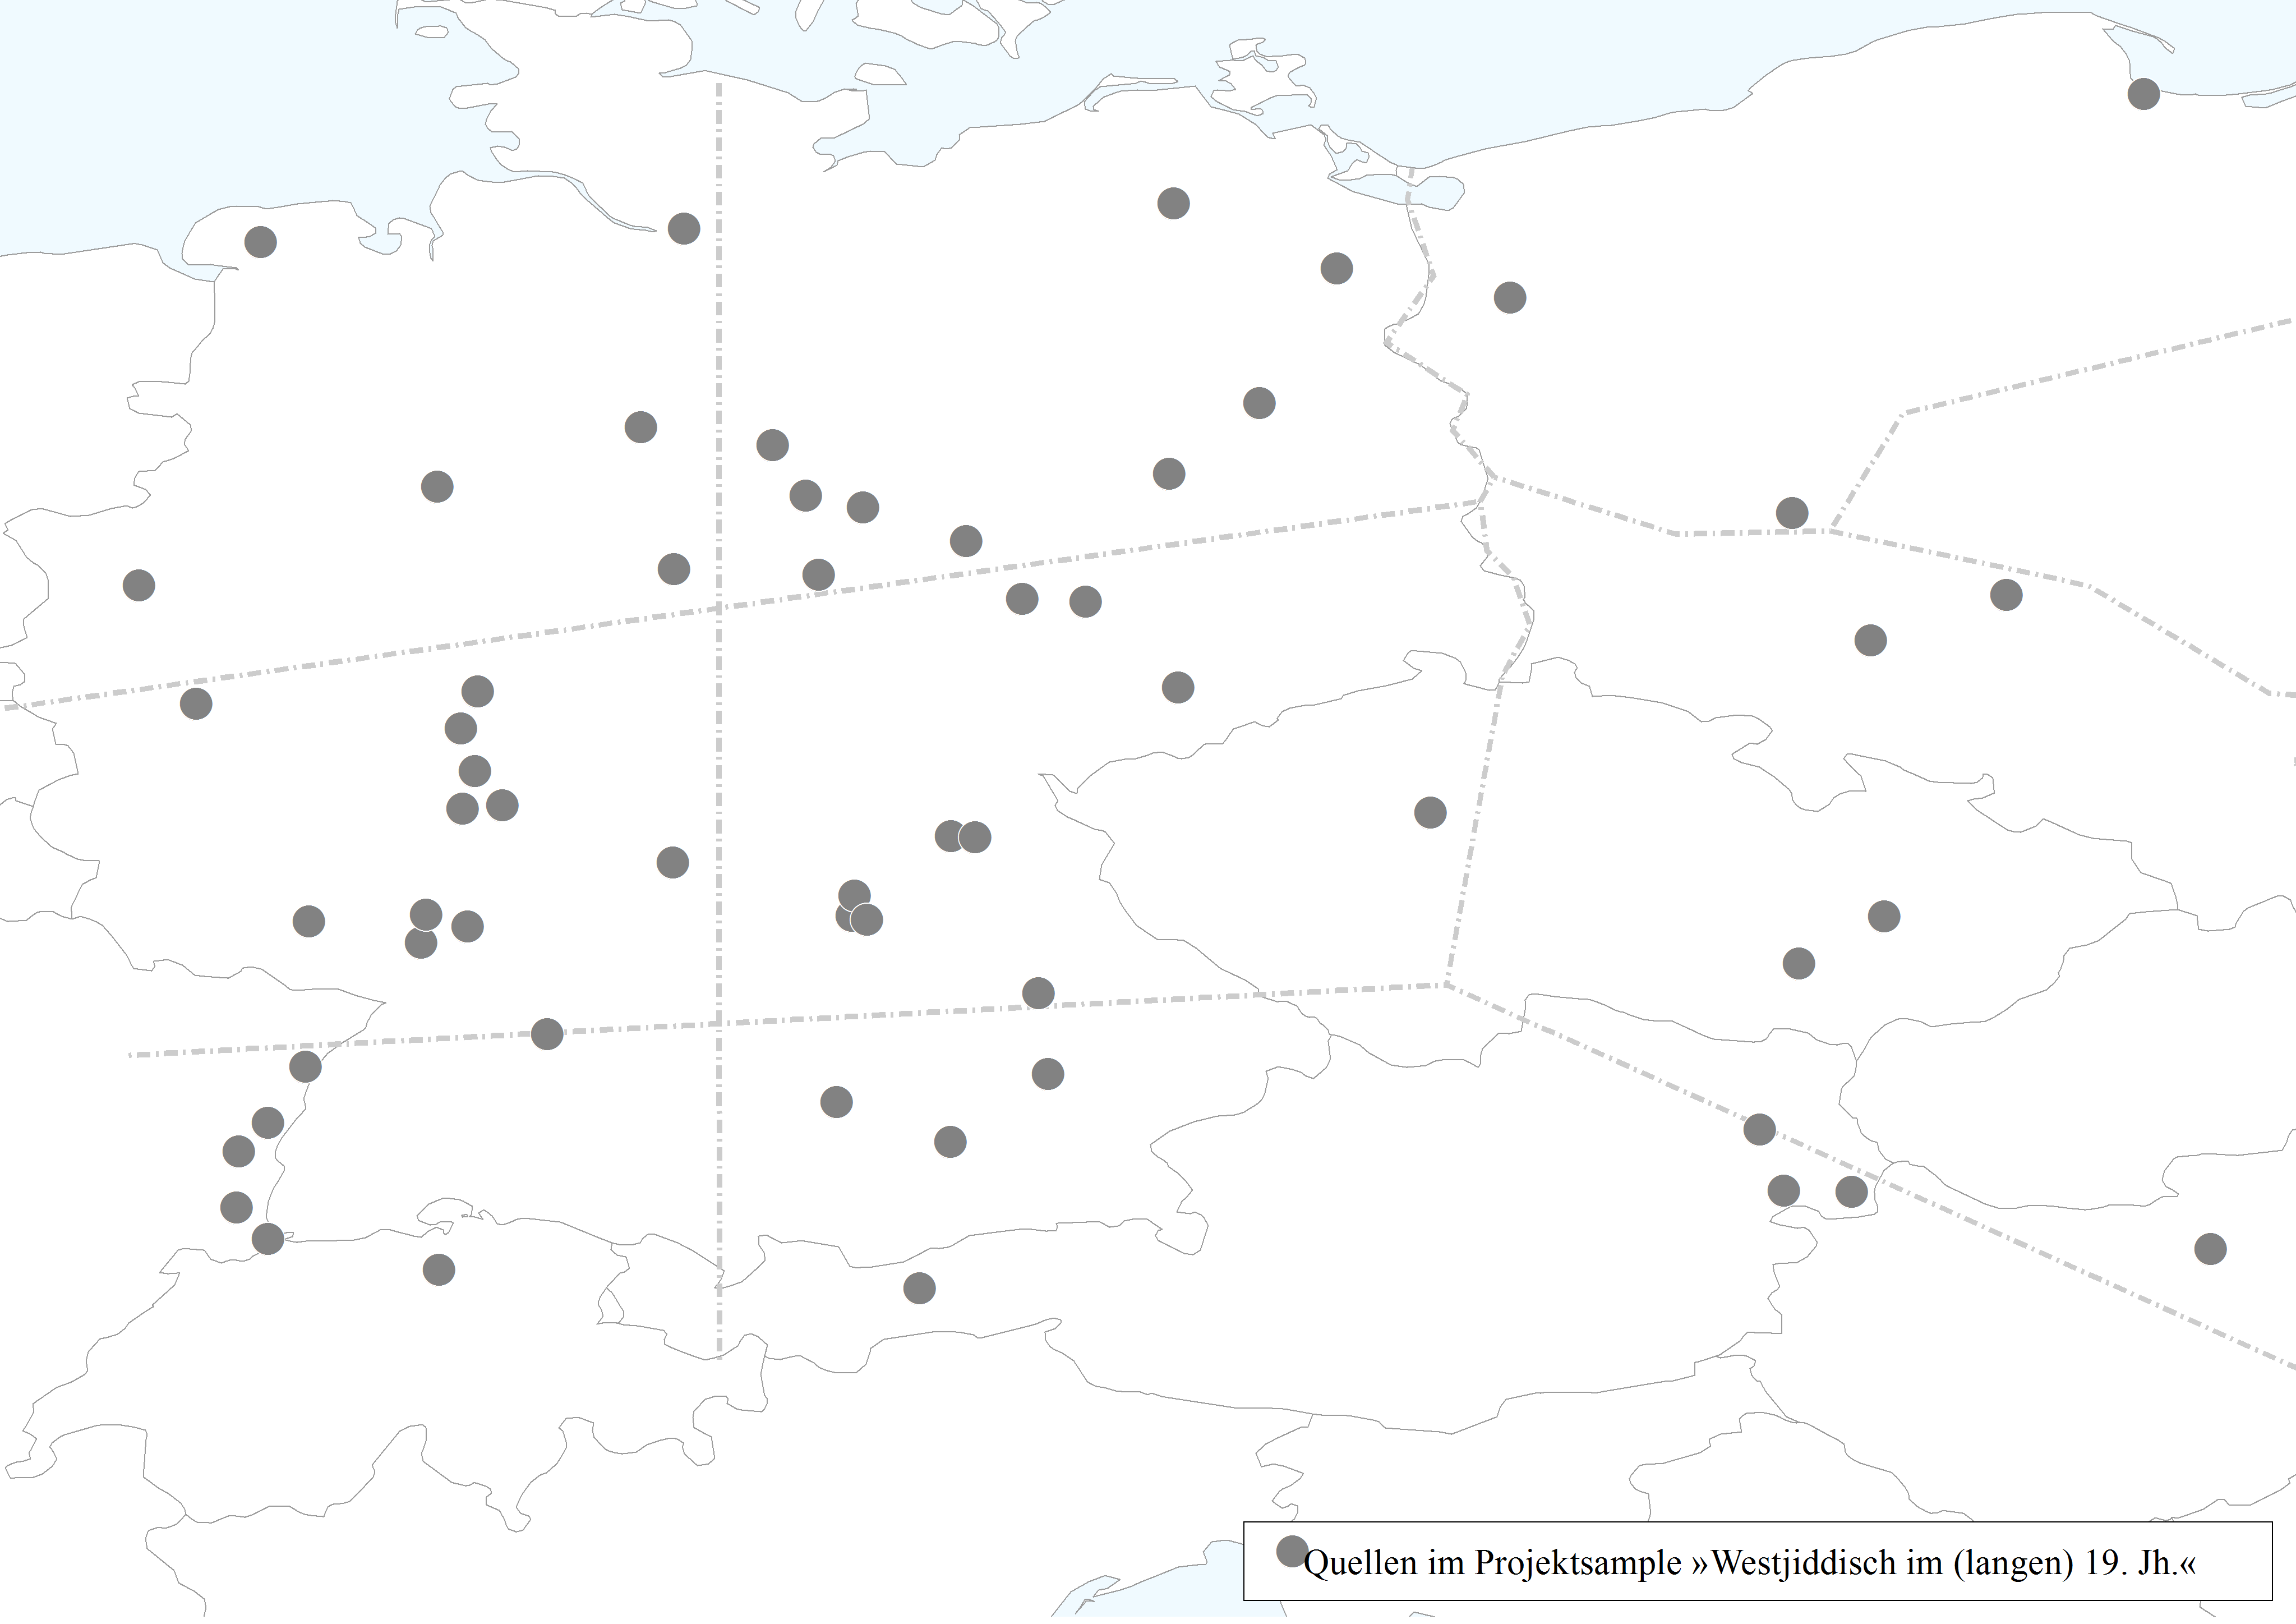
\includegraphics[width=\textwidth]{figures/quellengenerelldiss_sw.png}
		\caption{\label{kartegeo}Karte zur geographischen Verteilung des Projektsamples}
		\end{figure}
		\end{center}


%\noindent Die nachfolgenden  Beschreibungen der Westjiddischen Überlieferungsformen  (Kapitel \ref{Überlieferungsformen}) und der literarischen Verwendung des Jiddischen (Kapitel \ref{Kapitel Funktionstypen}) fußen auf den Ergebnissen des  Projektsamples, dessen aktuelle Version unter \url{http://www.online.uni-marburg.de/westjiddisch/index.php} einsehbar ist.  

Das Projektsample zeigt deutlich wie wichtig es ist den Wert nicht-jüdischer Quellen des späten Westjiddischen zu überprüfen, denn nur unter Zunahme dieses durchaus problematischen Datensatzes, ist es möglich quantitativ gesicherte Aussagen über sprachliche Strukturen des gesprochensprachlichen Westjiddischen zu treffen.


  \chapter{Untersuchungskorpus zum Literaturjiddischen} \label{korpora}
 % \epigraph{\textit{If you aren't taking a representative sample, you won't get a representative snapshot.}}{--- \textup{Nate Silver}}
% \epigraph{\textit{Any natural corpus will be skewed.}}{--- \cite[159]{Chomsky1957}}
% completes chomsky Zitat% \epigraph{\textit{Any natural corpus will be skewed. Some sentences won’t occur because they are obvious, others because they are false, still others because they are impolite. The corpus, if natural, will be so wildly skewed that the description would be no more than a mere list.}}{--- \textup{Noam Chomsky ([1957] 1962:159)}}
\noindent \ili{Literaturjiddisch} ist eine rein poetische  Varietät, keine natürliche Sprache. Obzwar es immer auf eine natürliche Sprache verweist (Jiddisch) und eingebettet ist in eine ebenfalls natürliche, wenn auch literarische Sprache (Deutsch), so unterscheidet sich ein \isi{Korpus}, bestehend aus literaturjiddischen Quellen, stark von anderen linguistischen Korpora. So ist in etwa der Vorwurf der Unvollständigkeit, den man jedem Textkorpus natürlicher Sprachen  vorhalten kann (vgl. insbes. \cite[159]{Chomsky1957}), im Falle des Literaturjiddischen haltlos: Über die literarische Überlieferung hinaus gibt es kein Zeugnis, da jenseits der Literatur kein \ili{Literaturjiddisch} bestehen kann. Jede literarische Figur eines jeden literarischen Textes legt uns bereits den Gesamtumfang ihrer Sprache dar. Aus linguistischer Perspektive haben wir es hierbei mit einem dankbaren Ausnahmefall zu tun. 

Die Recherchearbeit im Projekt \qu{Westjiddischen im (langen) 19. Jahrhundert} hat ergeben, dass \,%rs zum streichen
hauptsächlich literarische Quellen, zumeist Dramen, von vorwiegend christlichen Autoren überliefert sind (vgl.\, Abschnitt %linktomanuscript
\ref{sec:quellenkapitel}). Diese Texte entsprechen dem, was \cite{Richter1995} als \qu{Literaturjiddisch} definiert, da Jiddisch hier verschiedene literarische Funktionen trägt (vgl.\, Abschnitt \ref{Kapitel Funktionstypen}). Der Hauptfunktionstyp ist eine Mischform zwischen pejorativ und humoristisch (\hai{B2} \& \hai{C2}). Aufgrund dieser besonderen Datenlage besteht die Notwendigkeit, sich mit diesem speziellen Texttyp näher auseinanderzusetzen. Ausgehend von der im Projekt erarbeiteten Quellsammlung wurde gesondert ein \isi{Korpus} literaturjiddischer Texte der Typen \hai{B2}, \hai{C2} und \hai{D2} zusammengetragen und in Hinblick \,%rs r streichen
auf die darin vorkommenden sprachlichen Markierungen analysiert.\footnote{Da die Recherche nach literaturjiddischen Texten nicht im Zentrum des \hai{DFG}-Projekts stand, sondern die Recherche nach authentischen Quellen des Westjiddischen, erfasst das Projektsample wahrscheinlich einen geringen Ausschnitt dieses Quelltyps. Besonders aus der Mitte des 19. Jahrhunderts müssten noch deutlich mehr Quellen zu finden sein, als sie im Rahmen des Projektes erfasst wurden. Was diesen Quelltyp betrifft, sehen wir im Projektsample wohl nur die Spitze des Eisbergs. Für das Analysekorpus zum \hai{chrLiJi1} wurden zusätzliche Recherchen angestellt; dies gilt besonders für Fünfjahresintervalle, aus denen Quellen fehlten.} Dieses \isi{Korpus} zum christlichen \ili{Literaturjiddisch} im 19. Jahrhundert (\hai{chrLiJi1}) bildet das Kernkorpus dieser Arbeit.  

Die Texte des Kernkorpus haben gemeinsam, dass sie allesamt aus der Feder nicht-jüdischer Autoren stammen. Damit sind die darin auffindbaren Sprachdaten Information aus zweiter, wenn nicht sogar dritter Hand. Vorrangig aus diesem Grund wurde ein wesentlich kleineres Spezialkorpus zum \hai{jüdLiJi1} aufgebaut und analysiert (s. Abschnitt \,%rs Abschnitt ergänzen 
 \ref{spezialjüliji}). Ein solches macht darüber hinaus auch im Kontext einer diskursanalytischen Grundidee Sinn, da so geprüft werden kann, ob die Fremdwahrnehmung (\hai{chrLiJi1}) die Eigenwahrnehmung (\hai{jüdLiJi1}) beeinflusst oder nicht. 
  
  \section{Kernkorpus des nicht-jüdischen Literaturjiddischen im 19. Jahrhundert}\label{kernkorpus}
%\noindent
 Das Kernkorpus literaturjiddischer Texte der Funktionstypen \hai{B2}, \hai{C2} und \hai{D2} wurde nach folgenden Kriterien zusammengestellt:
 
 \begin{description}  
\item[\textbf{Diachrone} \textbf{Verteilung}] 
Auf der Zeitskala 1700–1950 wurden Fünfjahresintervalle gesetzt. Pro Intervall werden, sofern vorhanden, zwei Quellen analysiert.
\item [\textbf{Textsorte}] Dramen wurden bei der Auswahl bevorzugt, da diese zum einen unter den vorliegenden Textsorten den höchsten Grad konzeptioneller Mündlichkeit (nach \citealt{KochOesterreicher1985}) aufweisen, und da diese Textsorte zum anderen eine generell hohe Belegdichte aufweist. %linktomanuscript  (s. Abschnitt \ref{Verteilung Textsorten}).
\item [\textbf{Autorschaft}] Gesicherte nicht-jüdische Autorschaft.
\item [\textbf{Funktionstypen}] Es wurde versucht, das \isi{Korpus} in Bezug auf die Funktionstypen ausgewogen zu gestalten. Pro Intervall sollte je eine Quelle dem Typ \hai{B2} und eine dem Typ \hai{C2} angehören. Da eine Differenzierung zwischen \hai{B2} und \hai{C2} nicht immer einfach zu treffen ist, konnte dieses Kriterium nicht immer greifen. In dem Fall wurde versucht in einem Intervall mindestens eine Quelle, die eindeutig einem der beiden Typen \hai{B2} oder \hai{C2} zuzurechnen ist, aufzunehmen. Texte aus dem späten 19. und frühen 20. Jahrhundert dürfen auch dem \hai{D2}-Typ zugehören, sofern keine \hai{B2} oder \hai{C2} Quellen zur Verfügung standen. 
\item [\textbf{Sprechanteile jüdischer Figuren}] Sind pro Intervall mehrere potenzielle Quellen gegeben, werden die Quellen mit der höchsten Tokenfrequenz jüdischer Figurenrede gewählt.
\item[\textbf{Vermeidung gebundener Sprache}] Sofern es die Quellenlage erlaubt, werden Quellen in gebundener Sprache vermieden, da diese v.\,a.\, für die syntaktische Analyse u.\,U. ein verzerrendes Bild transportieren. 
\end{description}

Unberücksichtigt blieben bei der Korpusbildung die Faktoren der räumlichen Verteilung der Quellen und der Textlänge bzw. des Redeanteils jüdischer Figuren.\footnote{\label{FNSeitenzahlliji}Es wurde natürlich darauf Rücksicht genommen, Texte mit möglichst viel literaturjiddischen Sequenzen aufzunehmen, jedoch wurde das \isi{Korpus} nicht auf \quein{Normalseiten} (= 400 Wortformen pro Seite) skaliert (vgl.\, \qu{\citealt{Fnhdkorpus1972}} ). Die Zählung aller (physischen) \,%rs -n
 Seiten, die sprachlich relevante Daten zum \hai{chrLiJi1} liefern, ergab einen Gesamtumfang von 1181 Seiten. Eine durchschnittliche Quelle (Mittelwert) hat einen Umfang von 22,3 Seiten, liegt also grob betrachtet im Umfang der 30 Normalseiten, wie sie das \qu{Bonner Frühneuhochdeutschkorpus} verwendet. Wie man an der hohen Standardabweichung von 30,5 Seiten erkennt, ist das \isi{Korpus} extrem unausgewogen. Da die Texte in ihrem Umfang nicht skaliert wurden, sind Seitenzahlen generell weniger aussagekräftig und können keine Daten über die quantitative Verteilung eines Phänomens liefern. Die Angabe der Seitenzahlen erfüllt somit einen rein dokumentarischen Zweck, der die Korpusdaten überprüfbar macht.}  

Mit den angewandten Kriterien ist ein Textkorpus von 53 Texten entstanden, das zumindest den Zeitraum zwischen 1770 und 1875, immerhin 105 Jahre, lückenlos mit zwei Quellen abdeckt. Vor und nach diesem Zeitraum konnten nur vereinzelt relevante Texte in das \isi{Korpus} Eingang finden.
   
  \begin{figure}
\fittable{
	\begin{tikzpicture}
		\begin{axis}[ybar, width=1.02\textwidth,height=0.3\textheight,
		legend style={at={(1,1)},xshift=-13.25cm, yshift=-0.1cm,anchor=north west,nodes=left},
			%title={Funktionstypen des sp\"aten Westjiddisch},
			xtick={1700, 1725, 1750, 1775, 1800, 1825, 1850, 1875, 1900, 1925, 1950},
			x tick label style={ /pgf/number format/1000 sep=}, 
		y tick label style={/pgf/number format/1000 sep=},
			%extra y ticks={456.1, 1022.4},
			%extra y tick labels={{456,1},{1022,4}},
			extra y tick style={grid=major,
				tick label style={, ,}},
				ymin=0.1,
				bar width = 4pt,
				%ymax=5,
				ylabel={Quellen},
			enlarge x limits=0.03]		
			
				\addplot [fill=gray!20!white]  table [x=interval, y=kgesamt] {figures/kgesamt.txt};
						

			
			\legend{\hai{chrLiJi1}} %macht Legende
			
		\end{axis}			
	\end{tikzpicture}
}
	\caption{Quellenverteilung im \isi{Korpus} zum \hai{chrLiJi1}}\label{kgesamt}	
	\end{figure}



Ein Grund dafür, dass trotz intensiver Recherche vor 1770 und nach 1879 kaum Quellen vorliegen, kann sein, dass der sprachnormierende Diskurs über das Westjiddische in diesen Zeiten noch nicht bestand bzw. weitestgehend abgeschlossen war. Vom christlichen \ili{Literaturjiddisch} als eine kurzlebige \quein{Modeerscheinung} zu sprechen, ist, in Anbetracht der Datenlage, eine Untertreibung. Jüdische Figuren sprachlich zu markieren ist, wie Abschnitt \ref{westjiddistik} zeigt, ein über einen längeren Zeitraum etabliertes literarisches Mittel. Der Rückgang des Hebräischen zu Gunsten des Jiddischen als Zielsprache der \isi{Imitation} erlebt trotz vereinzelter Vorläufer in der ersten Jahrhunderthälfte des 18. Jahrhunderts erst ab den 1770ern seinen Durchbruch.%\footnote{Über die Recherchen im Projekt \qu{\ili{Westjiddisch} im (langen) 19. Jahrhunderts} hinaus, wurden zahlreiche Bemühungen angestellt, Texte des 16., 17., 18. und 20. Jahrhunderts ausfindig zu machen. Wie das \isi{Korpus} zeigt ohne viel Erfolg.} In dieser Zeit beginnt auch die Debatte um Sprachnormierung und die Aufgabe des Jiddischen zu Gunsten des Deutschen. Für die Zeit nach 1879 kann angenommen werden, dass \ili{Westjiddisch} bereits in den meisten Gegenden stark geschwunden ist. %Wie die Analyse der Quellen zeigt (s. Abschnitt \ref{analysen}), setzt hier allmählich ein Eindringen des Ostjiddischen in das \ili{Literaturjiddisch} ein, was den bereits fortgeschrittenen Rückgang des Westjiddischen in dieser Zeit bestätigen würde.   

Wie beabsichtigt machen Dramentexte den größten Anteil aus; jedoch mussten auch andere Textsorten und Quellen in gebundener Sprache aufgenommen werden (s. Tabelle \ref{tbltextsortenliji}). Für die Zeitabschnitte
 1725–1749 und 1840–1844 konnten nur lyrische Texte gefunden werden.
  
  
  %%Tablle chr\ili{LiJi1}
	\begin{table} 
	
		\begin{tabularx}{\textwidth}{ccccc}
		\lsptoprule
	  \textbf{Quellen (gesamt)}  &	 \textbf{Dramen} 	&  \textbf{Prosatexte}	&	\textbf{lyrische Texte}	&	\textbf{Sammlungen}	 \\ \midrule % horizontale Trennlinie
			  53 	&	34	&	6	&	9	&	4 \\
			 100\%  	&	64,15\% &	11,32\%	& 	16,98\%	&	7,55\%\\
			 \lspbottomrule
		 \end{tabularx}
		 \caption{\label{tbltextsortenliji}Textsorten im \isi{Korpus} zum \hai{chrLiJi1}}
		 
		 \end{table}
	 	


% \todo{Legende ragt in Diagramm hinein; Verlorener Satz zwischen Diagramm und Tabelle; Bekomme sie nicht bewegt :-O}
  %%%Diagramm gesamt korpus textsorten
  \begin{figure}[p]
\fittable{
	\begin{tikzpicture}
		\begin{axis}[cycle list name =linestyles*, width=0.9\textwidth,height=0.3\textheight,
		legend style={at={(1,1)},xshift=0.2cm, yshift=0cm,anchor=north west,nodes=left},
			%title={Funktionstypen des sp\"aten Westjiddisch},
			xtick={1700, 1725, 1750, 1775, 1800, 1825, 1850, 1875, 1900, 1925, 1950},
			x tick label style={ /pgf/number format/1000 sep=}, 
		y tick label style={/pgf/number format/1000 sep=},
			%extra y ticks={456.1, 1022.4},
			%extra y tick labels={{456,1},{1022,4}},
			extra y tick style={grid=major,
				tick label style={, ,}},
				ymin=0.1,
				%ymax=5,
				ylabel={Quellen},
			enlarge x limits=0.03]			
				\addplot [very thick] table [x=interval, y=kdramen] {figures/kdramen.txt};
		\addplot  [very thick, color=gray!40!white] table [x=interval, y=kprosa] {figures/kprosa.txt};
\addplot  [dotted, very thick] table [x=interval, y=ksammlung] {figures/ksammlung.txt};
\addplot  [dotted, very thick, color=gray!40!white] table [x=interval, y=klyrik] {figures/klyrik.txt};
		
			\legend{Dramen, Prosa, Sammlung, Lyrik} %macht Legende
				
		\end{axis}
	\end{tikzpicture}
}
	\caption{Diachrone Verteilung der Textsorten im \isi{Korpus} zum \hai{chrLiJi1}}
	\label{ktextsorte}	
	\end{figure}

Die diachrone Verteilung der Textsorten (Abbildung \ref{ktextsorte}) zeigt, dass sich zwischen 1770 und 1820 immerhin ein auf 25 Jahre erstreckendes Kontinuum ausschließlich dramatischer Quellen ergibt. Nach dieser Phase ist das \isi{Korpus} ein Gemisch verschiedener Textsorten. So lässt sich das \isi{Korpus} auf Grundlage % rs  auf Grundlage
der Textsortenverteilung in drei Abschnitte unterteilen:  im ersten Abschnitt (1700–1769) haben wir nur wenige, lyrische und epische Texte, in Abschnitt 2 (1770–1820) sind ausschließlich dramatische Quellen gegeben, während im dritten Abschnitt (1825–1949) eine große Textsortenvielfalt vorliegt. Dies muss bei der Analyse berücksichtigt werden.

 
Eine erneute, genauere Durchsicht der Texte ermöglichte eine Zuordnung der im Projektsample unter dem Mischtypus \hai{B2}/\hai{C2} laufenden Quellen als \hai{B2}- oder \hai{C2}-Quelle. Die Verteilung der Funktionstypen ist damit im Korpussample mehr oder weniger ausgeglichen (s. Tabelle \ref{tblfunktionstypenliji}). Die Typen \hai{B2} und \hai{C2} haben den größten Anteil. In nur drei Fällen musste auf Quellen des Typs \hai{D2} zurückgegriffen werden.\footnote{Diese drei Texte sind \hai{UT} (Stavenhagen, 1862), \hai{JD} (Wien, 1866) und \hai{AK} (Zürich, 1948).} In fünf Fällen konnte trotz intensiver Lektüre nicht entschieden werden, ob der \hai{B2}- oder der \hai{C2}-Typ vorliegt.\footnote{Dies betrifft die Quellen \hai{FL} (Mannheim, 1778), \hai{PF} (Augsburg, 1816), \hai{LP} (Brünn, 1849), \hai{FM} (Leipzig, 1852) und \hai{MV} (Berlin, 1862).}

 %%Tablle chr\ili{LiJi1} Funktionstypen
	\begin{table}[p]
	 
		\begin{tabularx}{\textwidth}{cCCCC}
		\lsptoprule
	\textbf{ Quellen (gesamt) } &	 \textbf{\hai{B2} }	&\textbf{ \hai{C2}}	&	\textbf{\hai{B2}} \& \textbf{\hai{C2}}	&	\textbf{\hai{D2}}	 \\ \midrule % horizontale Trennlinie
			  53 	&	24	&	21	&	5	&	3	 \\
			  100\% & 45,28\% & 39,62\% & 9,43\% & 5,66\% \\ 
\lspbottomrule
		 \end{tabularx}
		 \caption{\label{tblfunktionstypenliji} Verteilung der Funktionstypen im \isi{Korpus} zum \hai{chrLiJi1}}
		 
		 \end{table}
	 	

 
\begin{figure}[p]
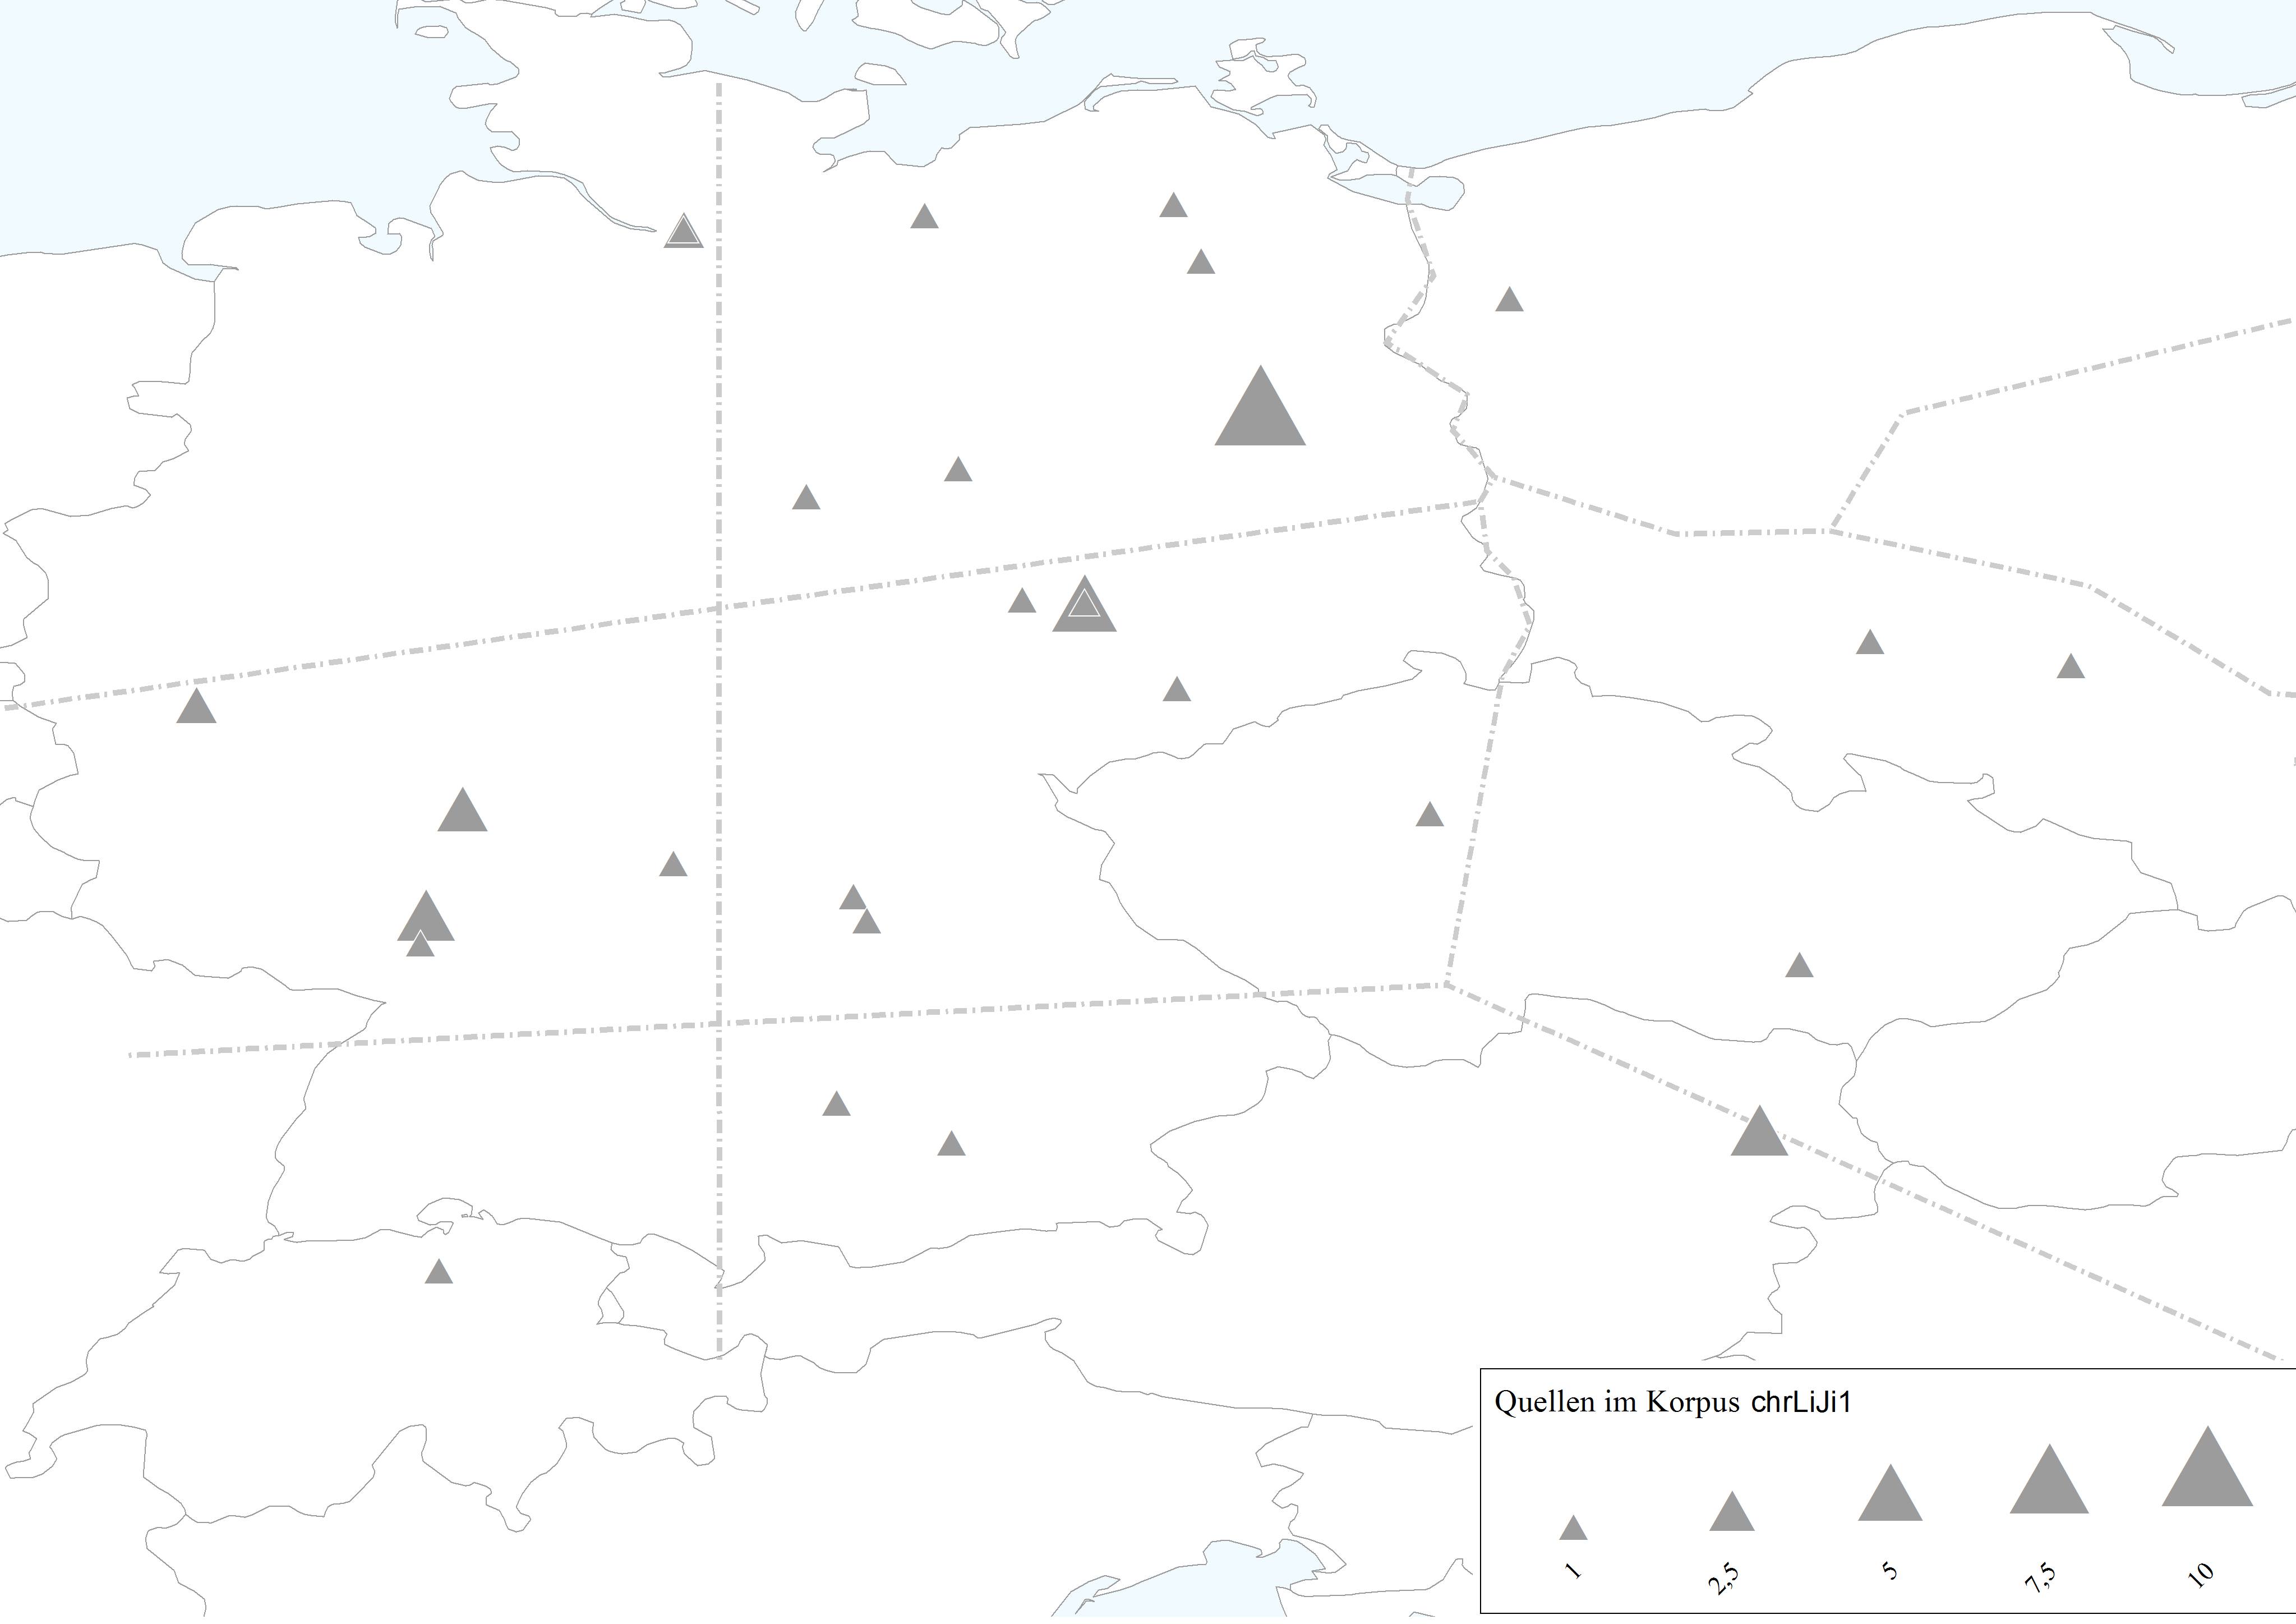
\includegraphics[width=\textwidth]{figures/liji1_menge3_diss_sw.png}
		\caption{\label{karteliji1menge} Karte zur quantitativen Verteilung des \isi{Korpus} \hai{chrLiJi1}}
		\end{figure}

 
Die räumliche Verteilung spielte bei der Korpusbildung keine Rolle. Wie die Kartierung der Korpusquellen zeigt (Abbildung \ref{karteliji1menge}),\footnote{Auch hier konnten nicht alle Texte einem Ort zugewiesen werden, vgl.\, Fn. \ref{FNkarte}, S.\, \pageref{FNkarte}. Insgesamt konnten 51 Quellen in die Kartierung aufgenommen werden.} entspricht dies der räumlichen Streuung des Projektsamples (vgl.\, Abbildung \ref{kartegeo}). Auch die quantitative Verteilung des \hai{chrLiJi1}-\isi{Korpus} (Abbildung \ref{karteliji1menge}) zeigt mit den Zentren Berlin, Leipzig, Wien, Frankfurt und Mannheim ähnliche Strukturen wie die des Projektsamples (vgl.\, \citealt[64, Abbildung 4.16]{SchaeferDiss}). Die im Projektsample besser abgedeckten Regionen des westl. \hai{{\NWJ}} und des nördlichen Übergangsgebiets sind im \hai{chrLiJi1}-\isi{Korpus} nur durch einzelne Quellen aus den Grenzgebieten repräsentiert. 





  
  %\clearpage
  Es sei erwähnt, dass in drei der aufgenommenen Texte Jiddisch nicht in Relation zum (Hoch-) Deutschen, sondern zu niederdeutschen Dialekten steht. Die entsprechenden Quellen sind \hai{UT} (Stavenhagen, 1862; Mecklenburgisch), \hai{DK} (Osterwieck, 1872; Ostfälisch) und \hai{DP} (Pyrzyce, 1874; westl. Ostpommersch). Die Analyse wird zeigen, ob in einer niederdeutschen Umgebung andere Strategien zur \isi{Emulation} des Jiddischen verwendet werden als in einer hochdeutschen.
  
Zwei Autoren sind im \isi{Korpus} mehrfach vertreten: Von Julius v. Voß wurden drei Dramen (\hai{EV} Berlin, 1817; \hai{NW} Berlin, 1804; \hai{PS} Berlin, 1808) und von Louis Angelt zwei Dramen (\hai{AJ} Berlin, 1825 u. \hai{PP} Berlin, 1839) ausgewertet. Dies könnte einerseits das Bild etwas verzerren, andererseits hat es den Vorteil, dass diese Autoren gesondert analysiert werden können, um zu prüfen, wie homogen sie sich im Textvergleich verhalten.\footnote{Wie die Clusteranalyse der Quellen zeigt (vgl. Abbildung \ref{boxplotcluster}, S. \pageref{boxplotcluster}), verhalten sich die jeweiligen Quellen trotz identischer Autorschaft unterschiedlich, was die Verteilung der verwendeten liji Phänomene betrifft. Ausgehend von dieser Clusteranalyse scheint auch die Matrixsprache (Hochdeutsch vs. Niederdeutsch) keinen entscheidenden Einfluss zu nehmen.}


 \section{Spezialkorpus des jüdischen \ili{Literaturjiddisch} im 19. Jahrhundert} \label{spezialjüliji}
%  %\noindent
 Um einen Eindruck zu erhalten, ob und wie der literarische Diskurs zum Jiddischen konfessionelle Unterschiede aufweist, wurde ein kleines Spezialkorpus zu literaturjiddischen Quellen jüdischer Autoren angelegt. Besonders interessant, da mit interkonfessioneller Leserschaft zu rechnen ist, sind Texte vom Funktionstyp \hai{C1}.\footnote{In zwei Fällen (PBerlin1 u. PBerlin2) besteht die Möglichkeit, dass diese Texte auch christlichen Autoren zuzuschreiben sind und damit dem Mischtyp \hai{C1}/\hai{C2} angehören. Diese Texte werden darum mit besonderer Vorsicht behandelt.} Darunter fallen fünf Bände der \qu{Gedichte und Scherze in jüdischer Mundart}\footnote{Von diesen Sammlungen jüdischer Witze und Anekdoten sind 23 Bände bekannt (vgl.\, \citealt{Gruschka2003}). Für das \isi{Korpus} wurden Bd. 1 und Bd. 23, sowie in Fünfer-Intervallen, die Bde. 5, 10 und 15 gewählt. Die zeitliche Verortung dieser Hefte ist jedoch heikel, da die Erstausgaben kaum mehr erhalten sind. Die Periode der Erstveröffentlichungen lässt sich auf den Zeitraum zwischen 1850 und 1870 eingrenzen. Bis in die 1870er Jahre hinein wurden die Hefte von Eduard Bloch in Berlin herausgegeben, dann aber nur mehr Reproduktionen.} und fünf Texte, die man als politische Pamphlete charakterisieren kann. Das \isi{Korpus} deckt den Zeitraum zwischen 1848 und 1877 ab.\footnote{Das \isi{Korpus} zum \hai{jüdLiJi1} umfasst 73 Seiten bei einem Mittelwert von 7 Seiten pro Quelle. Die Standardabweichung liegt bei 3 Seiten in einem noch relativ angemessenem Bereich (vgl.\, Fn. \ref{FNSeitenzahlliji} S.\, \pageref{FNSeitenzahlliji}).} Überwiegend haben diese Texte in Berlin ihren Ursprung bzw. waren im großstädtischen Raum verbreitet (\citealt{Gruschka2003}).\footnote{Die \hai{GuS} sind alle in Berlin gedruckt, ebenso die Pamphlete \hai{PBerlin1} und \hai{PBerlin2}. Die zahlreichen Pamphlete des Isaac Moses Hersch, von denen eines Eingang in das \isi{Korpus} gefunden hat (\hai{PAlsleben}), werden wahrscheinlich auch eher im großstädtischen Raum rezipiert worden sein als im Heimatort des Autors Alsleben. Die beiden weiteren Pamphlete stammen aus dem Gebiet des \hai{{\SÜJ}} mit Breslau (\hai{PBreslau}) und Debrecen (\hai{PDebrecen}). Letztere Quelle ist ein besonders interessantes Beispiel für ungarisches \hai{{\LiJi}}.}  	
    
  	\begin{table} 
 		\begin{tabular}{ccc}
\lsptoprule
	\textbf{Quellen (gesamt)  }&\textbf{GuS} 	&  \textbf{Pamphlete}	\\ 
\midrule 
			  10 	&	5	&	5	 \\
			  	&	ca.\, 1850er–1870er & 1848--1876\\ 
\lspbottomrule
		 \end{tabular}
		 \caption{\isi{Korpus} \hai{jüdLiJi1}}
		 \label{tbljüliji}
		 \end{table}
	 	
 Tatsächlich hätte ein \isi{Korpus} zum \hai{jüdLiJi1} deutlich umfangreicher ausfallen können. Dass hier nur zehn Texte Eingang gefunden haben, ist eindeutig nicht der Datenlage geschuldet, %linktomanuscript (vgl.\, Diagramm in Abbildung \ref{juedQuellen}), 
 sondern dem Fokus der Arbeit auf die \quein{\isi{Imitation} des Jiddischen} und dem literarischen Diskurs. Ziel der Korpora dieser Arbeit ist es nicht, möglichst authentische Quellen des Westjiddischen zusammenzutragen, sondern eben jene Quellen heranzuziehen, die besonders stark durch den kulturellen Diskurs beeinflusst  und damit möglichst weit entfernt von der Sprachwirklichkeit anzusiedeln sind. Die hier aufgenommenen Texte des \hai{jüdLiJi1} sind Quellen des assimilierten Judentums und Belege dafür, dass die \isi{Assimilation} nicht nur sprachlich, sondern auch formen- und literatursprachlich zur Jahrhunderthälfte stark fortgeschritten war.

  

                   
 \section{Methodik}\label{erhebungsmethode}


Die in den Korpora zusammengestellten Texte wurden einer Datenerhebung unterzogen, in welcher jeder Text händisch durchgegangen wurde und die darin vorkommenden sprachlichen Markierungen jüdischer Figurenrede in eine Phänomenmaske (s. Tabellen \ref{maske1} -- \ref{maske4}) eingetragen wurden.\footnote{Die in diese Maske aufgenommenen Phänomene ergeben sich aus den Daten selbst. Sie hat sich damit im Laufe der Datenerhebung herausgebildet und wurde nicht im \isi{Vorfeld} festgelegt. Aufgenommen wurde zunächst alles, was von der Schriftsprache abweicht. Die sprachlichen Abweichungen von der Literatursprache (Deutsch) mussten dazu selbstverständlich für mich selbst erkennbar und kategorisierbar und damit sprachwissenschaftlich \textit{salient} sein.} Zusätzlich wurden folgende Metadaten zu jedem Text angelegt:
 
 
 \begin{quote}
	 Titel [Kürzel],\footnote{Die Vergabe der Kürzel folgt der Regel: Quellen des christlichen \hai{{\LiJieins}} zwei Großbuchstaben, \hai{jüdLiJi1} Quellen der \qu{Gedichte und Scherze in jüdischer Mundart} als GuS+‘Nr. der jew. Ausgabe', Pamphlete des \hai{jüdLiJi1}-\isi{Korpus} werden mit P+‘Ort' abgekürzt. \,%rs Spatium fehlt
	Um einen leichteren Zugang zu ermöglichen, werden im Fließtext und in Sprachbeispielen die Kürzel zum \hai{chrLiJi1} um Erscheinungsort und Erscheinungsjahr ergänzt.\\
    Die Kürzel der untersuchten Quellen werden im Anhang (S. \pageref{appendixchrliji1}, \pageref{appendixjuedliji1}) %RS Klammer fehlt
 aufgeschlüsselt.} Autorenname, Erscheinungsjahr \\  Untertitel, Erscheinungsort, Verlag, Ausgaben 
Textsorte, Funktionstyp, Dia\-lektregion nach \cite{Katz1983} (falls ermittelbar)
Besondere Hinweise zu Inhalt u. Autor
 \end{quote}
		 
 Die Daten wurden bei der Eingabe in die Phänomenmaske auf maximal fünf Tokens pro Lexem (Lexik, Phonologie u. Graphie) bzw. pro Phänomen (im Fall von \isi{Morphologie} u. \isi{Syntax}) skaliert, so dass es möglich war, auch umfangreichere Texte aufzunehmen.  Ebenfalls der Skalierungsidee geschuldet ist der Umstand, dass jeder Beleg nur einmal pro Seite zitiert wurde, und zwar auch, wenn dieser mehr als einmal auf einer Seite vorliegt. Das heißt, jedes Datum ist mindestens einmal auf einer Seite belegt, die Belegzahlen sind aber nicht als absolute Werte zu verstehen. 
 
 Nicht erhoben wurden metasprachliche Laienurteile, wie z.\,B.\, in (\ref{bspmajorat}), da dieser Arbeit an der Erhebung grammatischer Formen der sprachlichen \isi{Imitation} gelegen ist und nicht an den sprachpolitischen Diskursen ums Jiddische.

 
  \eenumsentence{
	\item [] […] \textit{und nun erschallte hinter ihm ein fürchterliches Rabengekrächze aus dem Munde der alten Jüdin. In halb hebräischen Schimpfreden und im verzerrtesten Judendialekt zeihte sie die arme Tochter der Unkeuschheit,} […] \\ (\citealt[45]{Arnim1962}) 
\label{bspmajorat} 
}


Für das weitere Vorgehen wurden die Ergebnisse der Datenerhebung in das Programm \textsc{AntConc}\footnote{Diese Kon­kor­danz-Software wird unter \url{http://www.antlab.sci.waseda.ac.jp} zur freien Verfügung gestellt.} geladen und mit dessen Hilfe der näheren Analyse unterzogen. %Zur Darstellung der Analyseergebnisse werden im Folgenden Histogramme, Karten und Tabellen genutzt. 
Die erhobenen Daten aller Korpora finden sich im Appendix von \citet{SchaeferDiss}. %linktomanuscript
In den nachfolgenden Analysen der Einzelphänomene werden einzelne illustrierende Belege angeführt. Nur in einzelnen Fällen sind die im Text gegebenen Beispiele exhaustiv; in diesen Fällen wird dies explizit genannt. 

Die hier vorliegende Arbeit möchte einen ersten groben Überblick bieten, wie sprachliche \isi{Imitation} funktioniert. Demnach können in den Analysen singulär auftretende Einzelphänomene nur exemplarisch ausgewertet werden. Abstriche bei der Phänomenanalyse finden sich v.\,a.\, im lexikalischen Bereich und bei singulären phonologischen Phänomenen wieder. Prinzipiell wurde jedes Phänomen einer Detaillanalyse unterzogen, das in minimal vier Quellen des \hai{chrLiJi1} auftritt oder zumindest mit frequent auftretenden Manipulationsstrategien verwandt ist. 

\begin{table}
        \caption{Phänomenmaske Lexik}\label{maske1} 
        \begin{tabularx}{\textwidth}{lQQ}
	\lsptoprule
   &  \textbf{Phänomen}& \textbf{Beispiel}\\ 
\midrule 
	 	&Kennwörter {WJ} & \textit{Ette} \sem{Vater}, \textit{Mamme} \sem{Mutter}\\
 			& Kennwörter {OJ} & \textit{Tate} \sem{Vater}, \textit{Mame} \sem{Mutter} \\
 			& Hebraismen & \textit{Adonay} \sem{der Ewige}, \textit{Ische} \sem{Frau}\\
 			& Psychoostentative Ausdrücke & \textit{Wei geschrien!} \sem{Weh geschrien!}\\
 			& Sonstiges & \textit{heißt} \sem{nennt}, \textit{als} \sem{wie}\\
\lspbottomrule
\end{tabularx}
\end{table}

\begin{table} 
        \caption{Phänomenmaske Morphologie}\label{maske3} 
        \begin{tabularx}{\textwidth}{lQQ}
	\lsptoprule
    &  \textbf{Phänomen}& \textbf{Beispiel}\\ \midrule 
&	 {Diminution}\is{Diminution} (Singular; Plural) & \textit{Vögile} \sem{Vogel}, \textit{Madlich} \sem{Mädchen}\\
& Verbklasse \& Verbflexion & \textit{sennen} \sem{sie sind} \\
&Kasus bei vollen Obj.; Kasus n. Präp.; Kasus bei Pron.& \textit{Ich hob getroffen Menschen aus die ganze Welt } \sem{ich habe Menschen aus der ganzen Welt getroffen}\\
&Sonstiges&\textit{gespaziert} \sem{spaziert}\\ 
\lspbottomrule

\end{tabularx}
\end{table}

\begin{table}
        \caption{Phänomenmaske   Phonologie}\label{maske2} 
        \begin{tabularx}{\textwidth}{QQ}
	\lsptoprule
\hai{V24} (E\textsubscript{4} = {\mhd} \textit{ei}) > /a\textlengthmark/, /ɛ/ & \textit{Bahn} \sem{Bein}, \textit{kä} \sem{kein}\\
\tablevspace
\hai{V44} (O\textsubscript{4} = {\mhd} \textit{ou}) > /a\textlengthmark/ & \textit{kafen} \sem{kaufen}, \textit{Fra} \sem{Frau}\\
\textit{a}-Verdumpfung & \textit{hot} \sem{hat}, \textit{Tog} \sem{Tag}\\
\tablevspace
\hai{V22} (E\textsubscript{2} = {\mhd} \textit{ê}, \textit{œ}) > /ei/, /ai/ & \textit{seihe} \sem{sehe}, \textit{Keinik} \sem{König}\\
\tablevspace
\hai{V42} (O\textsubscript{2} = {\mhd} \textit{ô}) > /ou/, /au/& \textit{grous} \sem{groß}, \textit{waul} \sem{wohl}\\
\tablevspace
 \hai{V34} (I\textsubscript{4} = {\mhd} \textit{iu}) > <ei>, <ai>& \textit{neilich} \sem{neulich}, \textit{Leite} \sem{Leute}\\
\tablevspace
 Entrundungen (nhd. <ü>, <ö> > <i>, <e>)& \textit{ferchte} \sem{fürchte}, \textit{Mih} \sem{Mühe} \\
\tablevspace
{Palatalisierung}\is{Palatalisierung} /u\textlengthmark/ > /y/, /y\textlengthmark/& \textit{herüm} \sem{herum}, \textit{dü} \sem{du}\\ 
\tablevspace
Sproßvokal& \textit{Milich} \sem{Milch}\\
\tablevspace
<ai> für <ei>; <ey> für <ei>& \textit{haißt} \sem{heißt}, \textit{eyn} \sem{ein}\\
\tablevspace
ç > ʃ &\textit{nischt} \sem{nicht}\\
\tablevspace
<z> für <s>; <ß> für <s>; <ß> für <z>; <scht> für <st>& \textit{Zunne} \sem{Sonne}, \textit{ßag} \sem{sag}, \textit{ßu} \sem{zu}, \textit{Schtein} \sem{Stein}\\
\tablevspace
Konsonantismus \is{Konsonantismus} (diverses)& \textit{Köp} \sem{Kopf}, \textit{kegen} \sem{gegen}\\
\tablevspace
Sonstiges&\textit{schlage} \sem{schlagen}, \textit{et} \sem{es}\\
 \lspbottomrule
\end{tabularx}
\end{table}




\begin{table}
        \caption{Phänomenmaske Syntax}\label{maske4} 
        \begin{tabularx}{\textwidth}{QQ}
	\lsptoprule 
\hai{NP-Ex}; \hai{PP-Ex}; \hai{AP-Ex}; \hai{AdvP-Ex} & \textit{Bin ich gewesen in e Wein-Lokal} \sem{Bin ich in einem Weinlokal gewesen}\\
\tablevspace
\hai{VR} (zweigliedrig)& \textit{wo er soll essen} \sem{wo er essen soll}\\
\tablevspace
\hai{VR} (min. dreigliedrig)& \textit{as kein Buch darf vardorben werden} \sem{dass kein Buch verdorben werden darf}\\
\tablevspace
\hai{VPR}& \textit{daß er sich soll ahnen neien kahfen} \sem{dass er sich einen neuen kaufen soll}\\
\tablevspace
\hai{V2}& \textit{ass De bist still un ruhig} \sem{dass du still und ruhig bist}\\
\tablevspace
\hai{no-IPP}& \textit{Wie ich hob gewollt aheim gehen} \sem{Als ich habe heim gehen wollen}\\
\tablevspace
\isi{Relativpartikel}& \textit{ä Schnorrer, was is rumgelahfen in de Stadt} \sem{ein Bettler, der in der Stadt herumläuft}\\
\tablevspace
\isi{Negationskongruenz} \& -spreading & \textit{ber ßu sahnem Glicke hat's Kahner nicht gehert} \sem{zu seinem Glück hat es keiner gehört}\\
\tablevspace
\textit{kumen} + Bewegungsverb\textsubscript{\textit{zu}-Infinitiv}& \textit{Was kimmt ze geihn geritte?} \sem{Was kommt da geritten?}\\
\tablevspace
Sonstiges &\textit{eine Frage tun} \sem{fragen}\\
\lspbottomrule
\end{tabularx}
\end{table}
			